\documentclass{beamer}
\usepackage[utf8]{inputenc}
\usepackage{graphicx, epsfig}
\usepackage{amsmath,mathrsfs,amsfonts,amssymb}
\usepackage{floatflt}
\usepackage{epic,ecltree}
\usepackage{mathtext}
\usepackage{fancybox}
\usepackage{fancyhdr}
\usepackage{multirow}
\usepackage{enumerate}
\usepackage{epstopdf}
\usepackage{multicol}
\usepackage{algorithm}
\usepackage[noend]{algorithmic}
\usepackage{tikz}
\usepackage{blindtext}
\usetheme{default}%{Singapore}%{Warsaw}%{Warsaw}%{Darmstadt}
\usecolortheme{default}

\setbeamerfont{title}{size=\Huge}
\setbeamertemplate{footline}[page number]{}

\setbeamertemplate{section in toc}[sections numbered]


\makeatletter
\newcommand\HUGE{\@setfontsize\Huge{35}{40}}
\makeatother    

\setbeamerfont{title}{size=\HUGE}
\beamertemplatenavigationsymbolsempty

% latin bold lower
\newcommand{\ba}{\mathbf{a}} 
\newcommand{\bc}{\mathbf{c}} 
\newcommand{\be}{\mathbf{e}} 
\newcommand{\bh}{\mathbf{h}} 
\newcommand{\bp}{\mathbf{p}} 
\newcommand{\bt}{\mathbf{t}} 
\newcommand{\bs}{\mathbf{s}} 
\newcommand{\bu}{\mathbf{u}} 
\newcommand{\bv}{\mathbf{v}} 
\newcommand{\bw}{\mathbf{w}} 
\newcommand{\bx}{\mathbf{x}} 
\newcommand{\by}{\mathbf{y}} 
\newcommand{\bz}{\mathbf{z}} 

% latin bold upper
\newcommand{\bA}{\mathbf{A}} 
\newcommand{\bB}{\mathbf{B}} 
\newcommand{\bC}{\mathbf{C}} 
\newcommand{\bI}{\mathbf{I}} 
\newcommand{\bJ}{\mathbf{J}} 
\newcommand{\bL}{\mathbf{L}} 
\newcommand{\bM}{\mathbf{M}} 
\newcommand{\bP}{\mathbf{P}}
\newcommand{\bQ}{\mathbf{Q}} 
\newcommand{\bR}{\mathbf{R}} 
\newcommand{\bT}{\mathbf{T}} 
\newcommand{\bU}{\mathbf{U}} 
\newcommand{\bV}{\mathbf{V}} 
\newcommand{\bW}{\mathbf{W}} 
\newcommand{\bX}{\mathbf{X}} 
\newcommand{\bY}{\mathbf{Y}} 
\newcommand{\bZ}{\mathbf{Z}} 

% latin cal upper
\newcommand{\cF}{\mathcal{F}} 
\newcommand{\cG}{\mathcal{G}} 
\newcommand{\cI}{\mathcal{I}} 
\newcommand{\cL}{\mathcal{L}} 
\newcommand{\cM}{\mathcal{M}} 
\newcommand{\cN}{\mathcal{N}} 
\newcommand{\cP}{\mathcal{P}} 
\newcommand{\cS}{\mathcal{S}} 
\newcommand{\cT}{\mathcal{T}} 
\newcommand{\cW}{\mathcal{W}} 
\newcommand{\cX}{\mathcal{X}} 
\newcommand{\cZ}{\mathcal{Z}} 

% latin bb upper
\newcommand{\bbE}{\mathbb{E}} 
\newcommand{\bbI}{\mathbb{I}} 
\newcommand{\bbP}{\mathbb{P}} 
\newcommand{\bbR}{\mathbb{R}} 

% greek bold lower
\newcommand{\bepsilon}{\boldsymbol{\epsilon}} 
\newcommand{\btheta}{\boldsymbol{\theta}} 
\newcommand{\blambda}{\boldsymbol{\lambda}} 
\newcommand{\bpi}{\boldsymbol{\pi}} 
\newcommand{\bmu}{\boldsymbol{\mu}} 
\newcommand{\bsigma}{\boldsymbol{\sigma}} 
\newcommand{\bphi}{\boldsymbol{\phi}} 

% greek bold upper
\newcommand{\bSigma}{\boldsymbol{\Sigma}} 

\DeclareMathOperator*{\argmin}{arg\,min}
\DeclareMathOperator*{\argmax}{arg\,max}

\newcommand{\createdgmtitle}[1]{\title[\hbox to 56mm{Deep Generative Models  \hfill\insertframenumber\,/\,\inserttotalframenumber}]
	{\vspace{1cm} \\ \textbf{Deep Generative Models} \\ {\Huge Lecture #1}}
	\author{Roman Isachenko}
		\institute{
\includegraphics[width=0.7cm]{../utils/aimasterslogo} \LARGE{AI Masters}}
	\date{2024, Spring}
}

\usepackage{tikz}
\usetikzlibrary{arrows,shapes,positioning,shadows,trees}

\newcommand\myfootnote[1]{%
  \tikz[remember picture,overlay]
  \draw (current page.south west) +(1in + \oddsidemargin,0.5em)
  node[anchor=south west,inner sep=0pt]{\parbox{\textwidth}{%
      \rlap{\rule{10em}{0.4pt}}\raggedright\scriptsize \textit{#1}}};}

\newcommand\myfootnotewithlink[2]{%
  \tikz[remember picture,overlay]
  \draw (current page.south west) +(1in + \oddsidemargin,0.5em)
  node[anchor=south west,inner sep=0pt]{\parbox{\textwidth}{%
      \rlap{\rule{10em}{0.4pt}}\raggedright\scriptsize\href{#1}{\textit{#2}}}};}
      
\AtBeginSection[]
      {
      	\begin{frame}{Outline}
      		\tableofcontents[currentsection]
      	\end{frame}
      }
      \AtBeginSubsection[]{
      	\begin{frame}{Outline}
      		\tableofcontents[currentsection,currentsubsection]
      	\end{frame}
}
\createdgmtitle{9}
%--------------------------------------------------------------------------------
\begin{document}
%--------------------------------------------------------------------------------
\begin{frame}[noframenumbering,plain]
%\thispagestyle{empty}
\titlepage
\end{frame}
%=======
\begin{frame}{Recap of previous lecture}
	\begin{block}{Main problems of standard GAN}
		\begin{itemize}
			\item Vanishing gradients (solution: non-saturating GAN);
			\item Mode collapse (caused by Jensen-Shannon divergence).
		\end{itemize}
	\end{block}
	\begin{block}{Standard GAN}
		\vspace{-0.2cm}
		\[
		\min_{\btheta} \max_{\bphi} \left[ \bbE_{\pi(\bx)} \log D_{\bphi}(\bx) + \bbE_{p(\bz)} \log (1 - D_{\bphi}(\bG_{\btheta}(\bz))) \right]
		\]
		\vspace{-0.4cm}
	\end{block}
	\vspace{-0.1cm}
	\begin{block}{Informal theoretical results}
		The real images distribution $\pi(\bx)$ and the generated images distribution $p(\bx | \btheta)$ are low-dimensional and have disjoint supports. In this case
		\vspace{-0.3cm}
		\[
		KL(\pi || p) = KL(p || \pi) = \infty, \quad JSD(\pi || p) = \log 2.
		\]
	\end{block}
	\myfootnote{\href{https://arxiv.org/abs/1406.2661}{Goodfellow I. J. et al. Generative Adversarial Networks, 2014} \\
		\href{https://arxiv.org/abs/1701.04862}{Arjovsky M., Bottou L. Towards Principled Methods for Training Generative Adversarial Networks, 2017}}
\end{frame}
%=======
\begin{frame}{Recap of previous lecture}
	\begin{block}{Wasserstein distance}
		\vspace{-0.5cm}
		\[
		W(\pi, p) = \inf_{\gamma \in \Gamma(\pi, p)} \bbE_{(\bx, \by) \sim \gamma} \| \bx - \by \| =  \inf_{\gamma \in \Gamma(\pi, p)} \int \| \bx - \by \| \gamma (\bx, \by) d \bx d \by
		\]
		\vspace{-0.5cm}
		\begin{itemize}
			\item $\gamma(\bx, \by)$ -- transportation plan (the amount of "dirt" that should be transported from point $\bx$ to point $\by$).
			\item $\Gamma(\pi, p)$ -- the set of all joint distributions $\gamma (\bx, \by)$ with marginals $\pi$ and $p$ ($\int \gamma(\bx, \by) d \bx = p(\by)$, $\int \gamma(\bx, \by) d \by = \pi(\bx)$).
			\item $\gamma(\bx, \by)$ -- the amount, $\|\bx - \by \|$-- the distance.
		\end{itemize}
	\end{block}
	\begin{block}{Theorem (Kantorovich-Rubinstein duality)}
		\vspace{-0.2cm}
		\[
		W(\pi || p) = \frac{1}{K} \max_{\| f \|_L \leq K} \left[ \bbE_{\pi(\bx)} f(\bx)  - \bbE_{p(\bx)} f(\bx)\right],
		\]
		where $\| f \|_L \leq K$ are $K-$Lipschitz continuous functions ($f: \cX \rightarrow \bbR$).
	\end{block}
	\myfootnotewithlink{https://arxiv.org/abs/1701.07875}{Arjovsky M., Chintala S., Bottou L. Wasserstein GAN, 2017}
\end{frame}
%=======
\begin{frame}{Recap of previous lecture}
	\begin{block}{WGAN objective}
		\vspace{-0.3cm}
		\[
		\min_{\btheta} W(\pi || p) = \min_{\btheta} \max_{\bphi \in \boldsymbol{\Phi}} \left[ \bbE_{\pi(\bx)} f_{\bphi}(\bx)  - \bbE_{p(\bz)} f_{\bphi}(\bG_{\btheta}(\bz))\right].
		\]
		\vspace{-0.3cm}
	\end{block}
	\begin{itemize}
		\item Function~$f$ in WGAN is usually called $\textit{critic}$.
		\item If parameters $\bphi$ lie in a compact set $\boldsymbol{\Phi} \in [-c, c]^d$ then $f(\bx, \bphi)$ will be $K$-Lipschitz continuous function. 
	\end{itemize}
	\begin{multline*}
		K \cdot W(\pi || p) = \max_{\| f \|_L \leq K} \left[ \bbE_{\pi(\bx)} f(\bx)  - \bbE_{p(\bx)} f(\bx)\right] \geq \\  \geq \max_{\bphi \in \boldsymbol{\Phi}} \left[ \bbE_{\pi(\bx)} f_{\bphi}(\bx)  - \bbE_{p(\bx)} f_{\bphi}(\bx)\right]
	\end{multline*}
	\textit{"Weight clipping is a clearly terrible way to enforce a Lipschitz constraint"}
	\myfootnotewithlink{https://arxiv.org/abs/1701.07875}{Arjovsky M., Chintala S., Bottou L. Wasserstein GAN, 2017}
\end{frame}
%=======
\begin{frame}{Recap of previous lecture}
	\begin{block}{Theorem}
		Let $\pi(\bx)$ and $p(\bx)$ be two distribution in $\cX$, a compact metric space. Let $\gamma$ be the optimal transportation plan between $\pi(\bx)$ and $p(\bx)$. Then
		\vspace{-0.4cm}
		\[
			\bbP_{(\by, \bz) \sim \gamma} \left[ \nabla f^*(\hat{\bx}_t) = \frac{\bz - \hat{\bx}_t}{\| \bz - \hat{\bx}_t \|} \right] = 1.
		\]
		\vspace{-0.6cm}
	\end{block}
	\begin{block}{Gradient penalty}
		\vspace{-0.5cm}
		\[
			W(\pi || p) = \underbrace{\bbE_{\pi(\bx)} f(\bx)  - \bbE_{p(\bx)} f(\bx)}_{\text{original critic loss}} + \lambda \underbrace{\bbE_{U[0, 1]} \left[ \left( \| \nabla f(\hat{\bx}) \|_2 - 1 \right) ^ 2\right]}_{\text{gradient penalty}}.
		\]
		\vspace{-0.5cm}
	\end{block}
	Samples $\hat{\bx}_t = t \cdot \by + (1 - t) \cdot \bz$ with $t \in [0, 1]$ are uniformly sampled along straight lines between pairs of points: $\by \sim \pi(\bx)$ and $\bz \sim p(\bx | \btheta)$.
	\myfootnote{
	\href{https://arxiv.org/abs/1701.07875}{Arjovsky M., Chintala S., Bottou L. Wasserstein GAN, 2017} \\
	\href{https://arxiv.org/abs/1704.00028}{Gulrajani I. et al. Improved Training of Wasserstein GANs, 2017} }
\end{frame}
%=======
\begin{frame}{Recap of previous lecture}
	\vspace{-0.3cm}
	\begin{block}{f-divergence minimization}
		\vspace{-0.3cm}
		\[
			D_f(\pi || p) = \bbE_{p(\bx)}  f\left( \frac{\pi(\bx)}{p(\bx)} \right) \rightarrow \min_p.
		\]
		Here $f: \bbR_+ \rightarrow \bbR$ is a convex, lower semicontinuous function satisfying $f(1) = 0$.
	\end{block}
	\begin{block}{Variational divergence estimation}
		\vspace{-0.3cm}
		\[
			D_f(\pi || p) \geq \sup_{T \in \cT} \left[\bbE_{\pi}T(\bx) -  \bbE_p f^*(T(\bx)) \right],
		\]
		\vspace{-0.7cm}
	\end{block}
	\begin{block}{Fenchel conjugate}
		\vspace{-0.7cm}
		\[
		f^*(t) = \sup_{u \in \text{dom}_f} \left( ut - f(u) \right), \quad f(u) = \sup_{t \in \text{dom}_{f^*}} \left( ut - f^*(t) \right)
		\]
		\vspace{-0.5cm}
	\end{block}
	\textbf{Note:} To evaluate lower bound we only need samples from $\pi(\bx)$ and $p(\bx)$. Hence, we could fit implicit generative model.
	\myfootnotewithlink{https://arxiv.org/abs/1606.00709}{Nowozin S., Cseke B., Tomioka R. f-GAN: Training Generative Neural Samplers using Variational Divergence Minimization, 2016}
\end{frame}
%=======
\begin{frame}{Outline}
	\tableofcontents
\end{frame}
%=======
\section{Evaluation of likelihood-free models}
%=======
\begin{frame}{Evaluation of likelihood-free models}
	How to evaluate generative models?
	\begin{block}{Likelihood-based models}
		\begin{itemize}
			\item Split data to train/val/test.
			\item Fit model on the train part.
			\item Tune hyperparameters on the validation part.
			\item Evaluate generalization by reporting likelihoods on the test set.
		\end{itemize}
	\end{block}
	\begin{block}{Not all models have tractable likelihoods}
		\begin{itemize}
			\item VAE: compare ELBO values.
			\item GAN: ???
		\end{itemize}
	\end{block}
\end{frame}
%=======
\begin{frame}{Evaluation of likelihood-free models}
	Let take some pretrained image classification model to get the conditional label distribution $p(y | \bx)$ (e.g. ImageNet classifier).
	\begin{block}{What do we want from samples?}
		\begin{itemize}
			\item \textbf{Sharpness}
			\begin{figure}
				\centering
				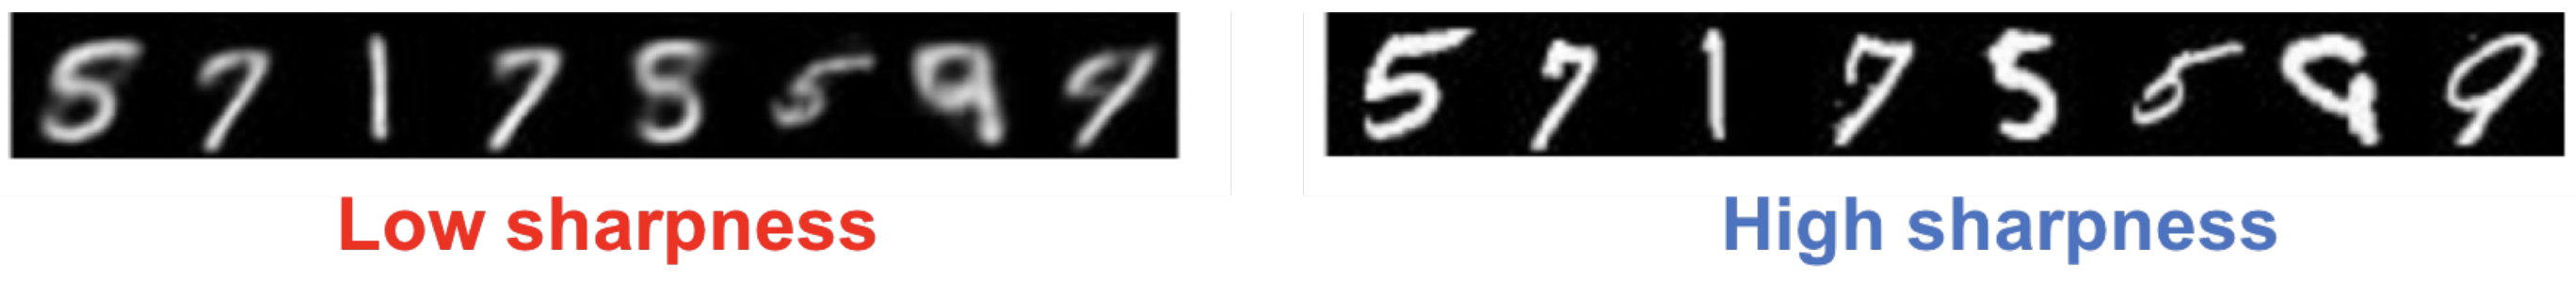
\includegraphics[width=0.9\linewidth]{figs/sharpness}
			\end{figure}
			The conditional distribution $p(y | \bx)$ should have low entropy (each image $\bx$ should have distinctly recognizable object).
			\item \textbf{Diversity}
			\begin{figure}
				\centering
				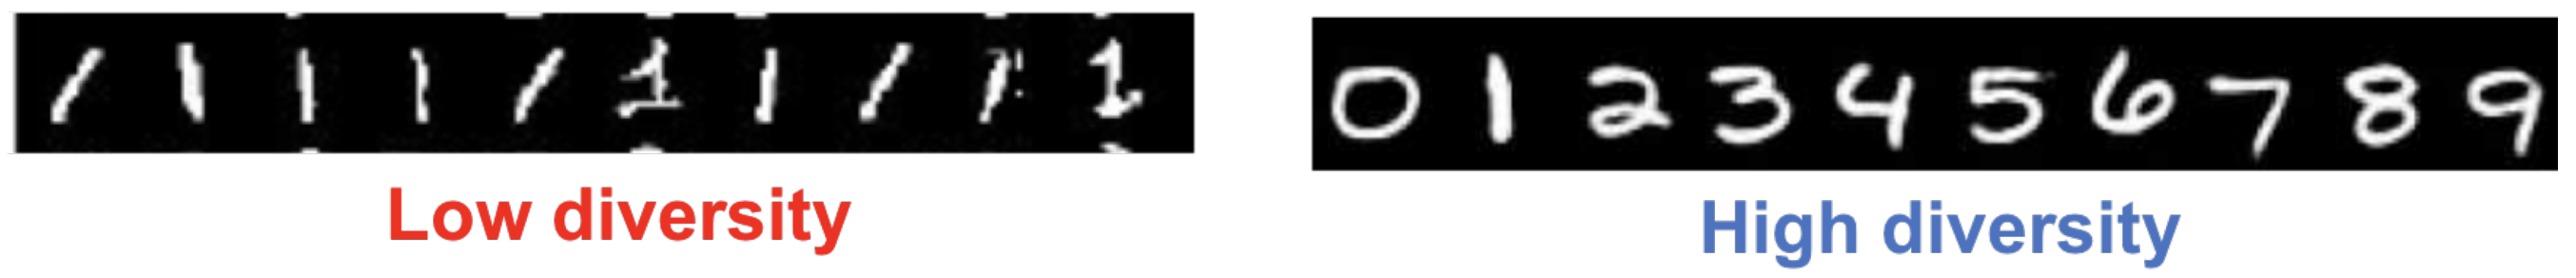
\includegraphics[width=0.9\linewidth]{figs/diversity}
			\end{figure}
			The marginal distribution $p(y) = \int p(y | \bx) p(\bx) d \bx$ should have high entropy (there should be as many classes generated as possible).
		\end{itemize}
	\end{block}
	\myfootnotewithlink{https://deepgenerativemodels.github.io}{image credit: https://deepgenerativemodels.github.io}
\end{frame}
%=======
\subsection{Frechet Inception Distance (FID)}
%=======
\begin{frame}{Frechet Inception Distance (FID)}
	\begin{block}{Wasserstein metric}
		\vspace{-0.2cm}
		\[
		W_s(\pi, p) = \inf_{\gamma \in \Gamma(\pi, p)} \left(\bbE_{(\bx, \by) \sim \gamma} \| \bx - \by \|^s\right)^{1/s}
		\]
		\vspace{-0.6cm}
	\end{block}
	\begin{block}{Theorem}
		If $\pi(\bx) = \cN(\bmu_\pi, \bSigma_\pi)$, $p(\by) = \cN(\bmu_p, \bSigma_p)$, then
		\vspace{-0.3cm}
		\[
		W_2^2(\pi, p) = \| \bmu_{\pi} - \bmu_{p}\|_2^2 + \text{tr} \left[ \bSigma_{\pi} + \bSigma_p - 2 \left(\bSigma_{\pi}^{1/2} \bSigma_p \bSigma_{\pi}^{1/2} \right)^{1/2} \right]
		\]
		\vspace{-0.7cm}
	\end{block}
	\begin{block}{Frechet Inception Distance}
		\vspace{-0.3cm}
		\[
			\text{FID} (\pi, p) =  W_2^2(\pi, p)
		\]
		\vspace{-0.6cm}
	\end{block}
	\begin{itemize}
		\item Representations are the outputs of the intermediate layer from the pretrained classification model.
		\item $\bmu_{\pi}$, $\bSigma_{\pi}$ and $\bmu_{p}$, $\bSigma_p$ are the statistics of the feature representations for the samples from $\pi(\bx)$ and $p(\bx | \btheta)$.
	\end{itemize}
	\myfootnotewithlink{https://arxiv.org/abs/1706.08500}{Heusel M. et al. GANs Trained by a Two Time-Scale Update Rule Converge to a Local Nash Equilibrium, 2017}
\end{frame}
%=======
\begin{frame}{Frechet Inception Distance (FID)}
	\vspace{-0.4cm}
	\[
	\text{FID} (\pi, p) =  \| \bmu_{\pi} - \bmu_{p}\|_2^2 + \text{tr} \left[ \bSigma_{\pi} + \bSigma_p - 2 \left(\bSigma_{\pi}^{1/2} \bSigma_p \bSigma_{\pi}^{1/2} \right)^{1/2} \right]
	\]
	\vspace{-0.3cm}
	\begin{itemize}
		\item Needs a large sample size for evaluation.
		\item Calculation of FID is slow.
		\item High dependence on the pretrained classification model.
		\item Uses the normality assumption!
	\end{itemize}
	\begin{figure}
		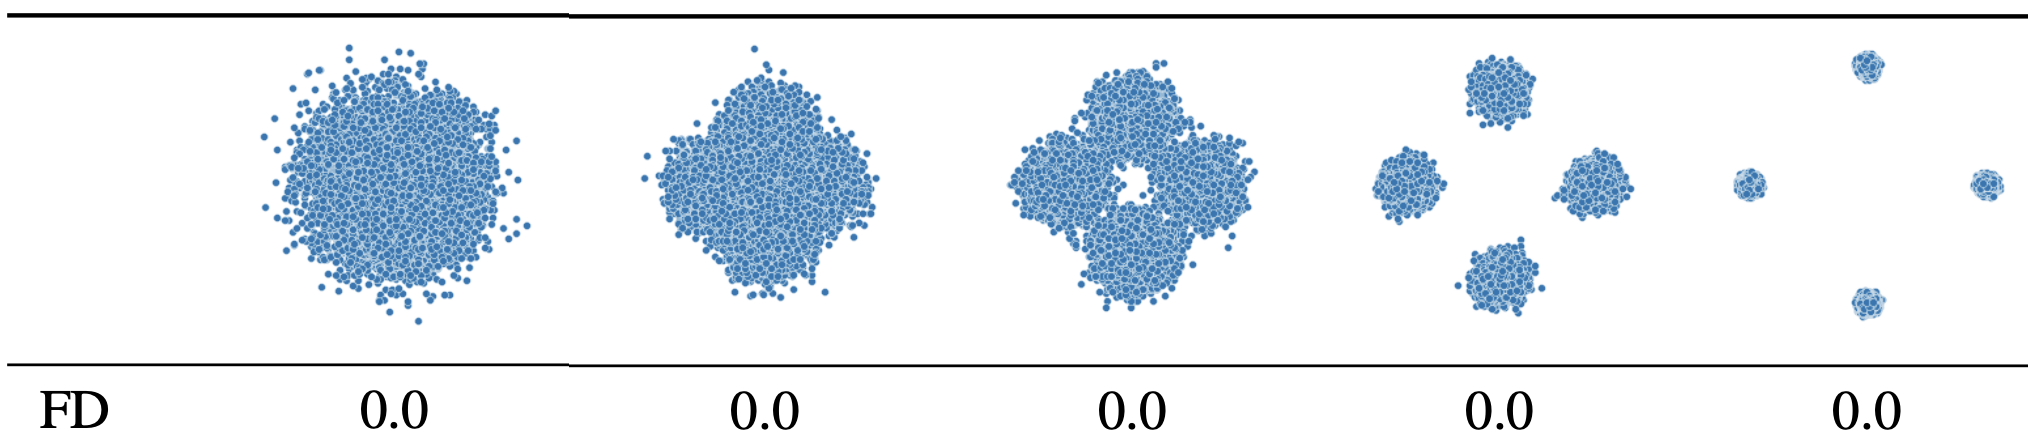
\includegraphics[width=0.95\linewidth]{figs/fid_normal}
	\end{figure}
	
	\myfootnotewithlink{https://arxiv.org/abs/2401.09603}{Jayasumana S. et al. Rethinking FID: Towards a Better Evaluation Metric for Image Generation, 2024}
\end{frame}
%=======
\subsection{Maximum Mean Discrepancy (MMD)}
%=======
\begin{frame}{Maximum Mean Discrepancy (MMD)}
	\begin{block}{Theorem}
		$\pi(\bx) = p(\by)$ if and only if $\bbE_{\pi(\bx)} f(\bx) = \bbE_{p(\by)} f(\by)$ for any bounded and continuous $f$.
	\end{block}
	\vspace{-0.3cm}
	\[
		\text{MMD}(\pi, p) = \sup_f \left[ \bbE_{\pi(\bx)} f(\bx) - \bbE_{p(\bx)} f(\bx) \right]
	\]	
	\vspace{-0.3cm}
	\begin{block}{Theorem (Reproducing Kernel Hilbert Space)}
		\vspace{-0.6cm}
		\[
			\text{MMD}^2(\pi, p) = \bbE_{\substack{\bx \sim\pi(\bx) \\ \bx' \sim\pi(\bx)}} k(\bx, \bx') + \bbE_{\substack{\by \sim p(\by) \\ \by' \sim p(\by)}} k(\by, \by') - 2 \bbE_{\substack{\bx \sim\pi(\bx) \\ \by \sim p(\by)}} k(\bx, \by)
		\]
		\begin{itemize}
			\item $k(\bx, \by)$ is a positive definite, symmetric kernel function (for example $k(\bx, \by) = \frac{\exp(\|\bx - \by\|^2)}{\sigma^2}$);
			\item $f(\bx) = \langle f, \phi(\bx) \rangle_{\mathcal{H}}$;
			\item $\phi(\bx) = k(\cdot, \bx)$.
		\end{itemize} 
		\vspace{-0.3cm}
	\end{block}
	\myfootnotewithlink{https://arxiv.org/abs/2401.09603}{Jayasumana S. et al. Rethinking FID: Towards a Better Evaluation Metric for Image Generation, 2024}
\end{frame}
%=======
\begin{frame}{Maximum Mean Discrepancy (MMD)}
		\vspace{-0.6cm}
		\[
			\text{MMD}^2(\pi, p) = \bbE_{\substack{\bx \sim\pi(\bx) \\ \bx' \sim\pi(\bx)}} k(\bx, \bx') + \bbE_{\substack{\by \sim p(\by) \\ \by' \sim p(\by)}} k(\by, \by') - 2 \bbE_{\substack{\bx \sim\pi(\bx) \\ \by \sim p(\by)}} k(\bx, \by)
		\]
		\vspace{-0.3cm}
	\begin{figure}
		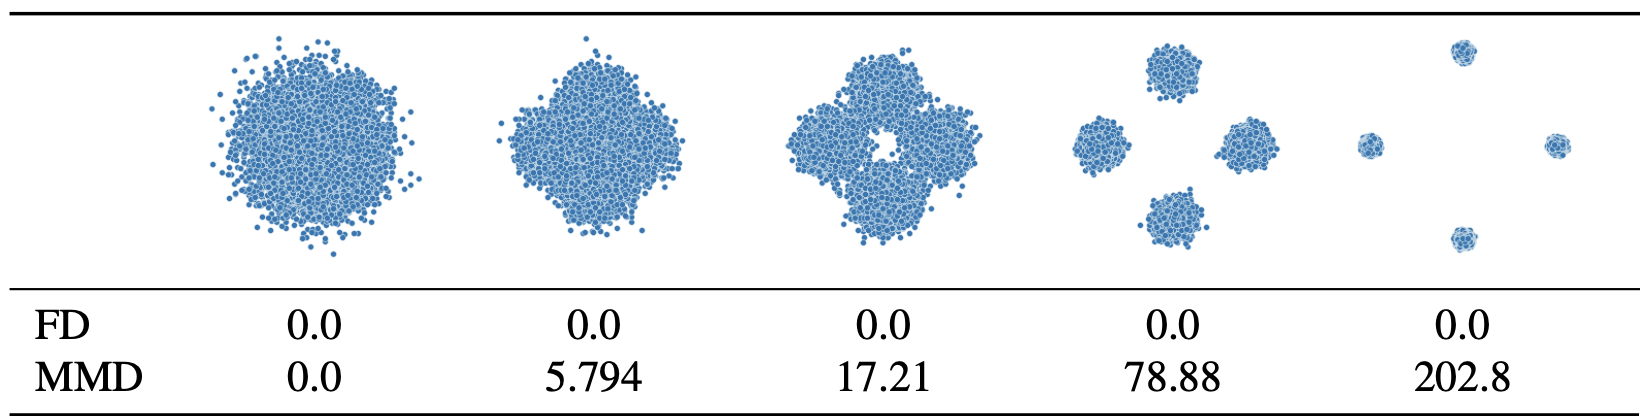
\includegraphics[width=0.95\linewidth]{figs/mmd_normal}
	\end{figure}
	\begin{itemize}
		\item Needs less sample size for evaluation.
		\item High dependence on the pretrained classification model.
		\item Works with any distribution!
	\end{itemize}
	\myfootnotewithlink{https://arxiv.org/abs/2401.09603}{Jayasumana S. et al. Rethinking FID: Towards a Better Evaluation Metric for Image Generation, 2024}
\end{frame}
%=======
\subsection{Precision-Recall}
%=======
\begin{frame}{Precision-Recall}
	\begin{block}{What do we want from samples}
		\begin{itemize}
			\item \textbf{Sharpness}: generated samples should be of high quality.
			\item \textbf{Diversity}: their variation should match that observed in the training set.
		\end{itemize}
	\end{block}
	\vspace{-0.5cm}
	\begin{figure}
		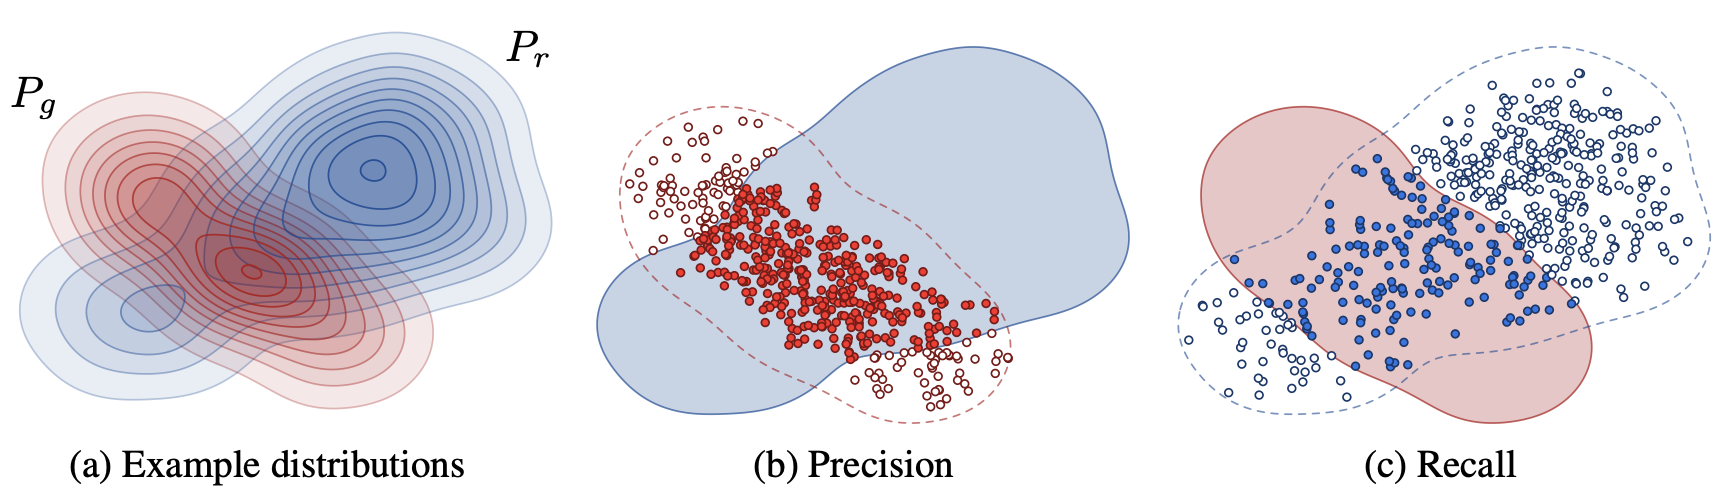
\includegraphics[width=0.95\linewidth]{figs/pr_curve}
	\end{figure}
	\vspace{-0.3cm}
	\begin{itemize}
		\item \textbf{Precision} denotes the fraction of generated images that are realistic.
		\item \textbf{Recall} measures the fraction of the training data manifold covered by the generator.
	\end{itemize}
	\myfootnotewithlink{https://arxiv.org/abs/1904.06991}{Kynkäänniemi T. et al. Improved precision and recall metric for assessing generative models, 2019}
\end{frame}
%=======
\begin{frame}{Precision-Recall}
	\begin{itemize}
		\item $\cS_{\pi} = \{\bx_i\}_{i=1}^{n} \sim \pi(\bx)$ -- real samples;
		\item $\cS_{p} = \{\bx_i\}_{i=1}^{n} \sim p(\bx | \btheta)$ -- generated samples.
	\end{itemize}
	Embed samples using pretrained classifier network (as previously):
	\[
		\cG_{\pi} = \{\mathbf{g}_i\}_{i=1}^n, \quad \cG_{p} = \{\mathbf{g}_i\}_{i=1}^n.
	\]
	Define binary function:
	\[
		f(\mathbf{g}, \cG) = 
		\begin{cases}
			1, \quad \text{if exists } \mathbf{g}' \in \cG: \| \mathbf{g}  - \mathbf{g}'\|_2 \leq \| \mathbf{g}' - \text{NN}_k(\mathbf{g}', \cG)\|_2; \\
			0, \quad \text{otherwise.}
		\end{cases}
	\]
	\[
		\text{Precision} (\cG_{\pi}, \cG_{p}) = \frac{1}{n} \sum_{\mathbf{g} \in \cG_{p}} f(\mathbf{g}, \cG_{\pi}); \,\, \text{Recall} (\cG_{\pi}, \cG_{p}) = \frac{1}{n} \sum_{\mathbf{g} \in \cG_{\pi}} f(\mathbf{g}, \cG_{p}).
	\]
	\vspace{-0.4cm}
	\begin{figure}
		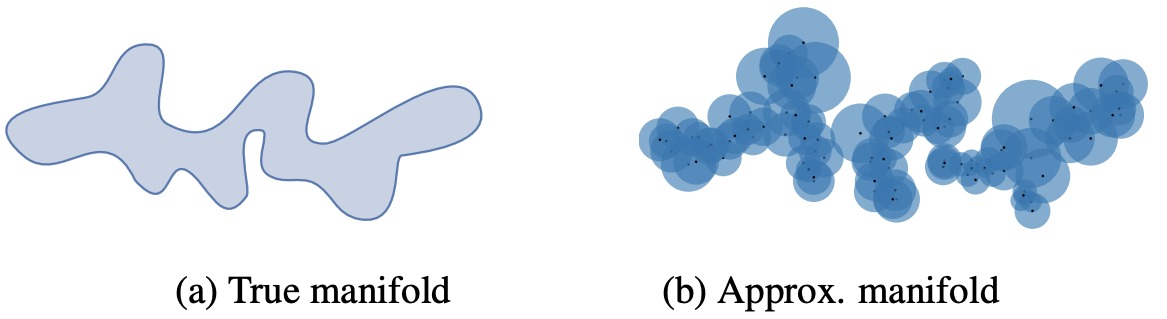
\includegraphics[width=0.7\linewidth]{figs/pr_k_nearest}
	\end{figure}
	\myfootnotewithlink{https://arxiv.org/abs/1904.06991}{Kynkäänniemi T. et al. Improved precision and recall metric for assessing generative models, 2019}
\end{frame}
%=======
\begin{frame}{Precision-Recall}
	\begin{figure}
		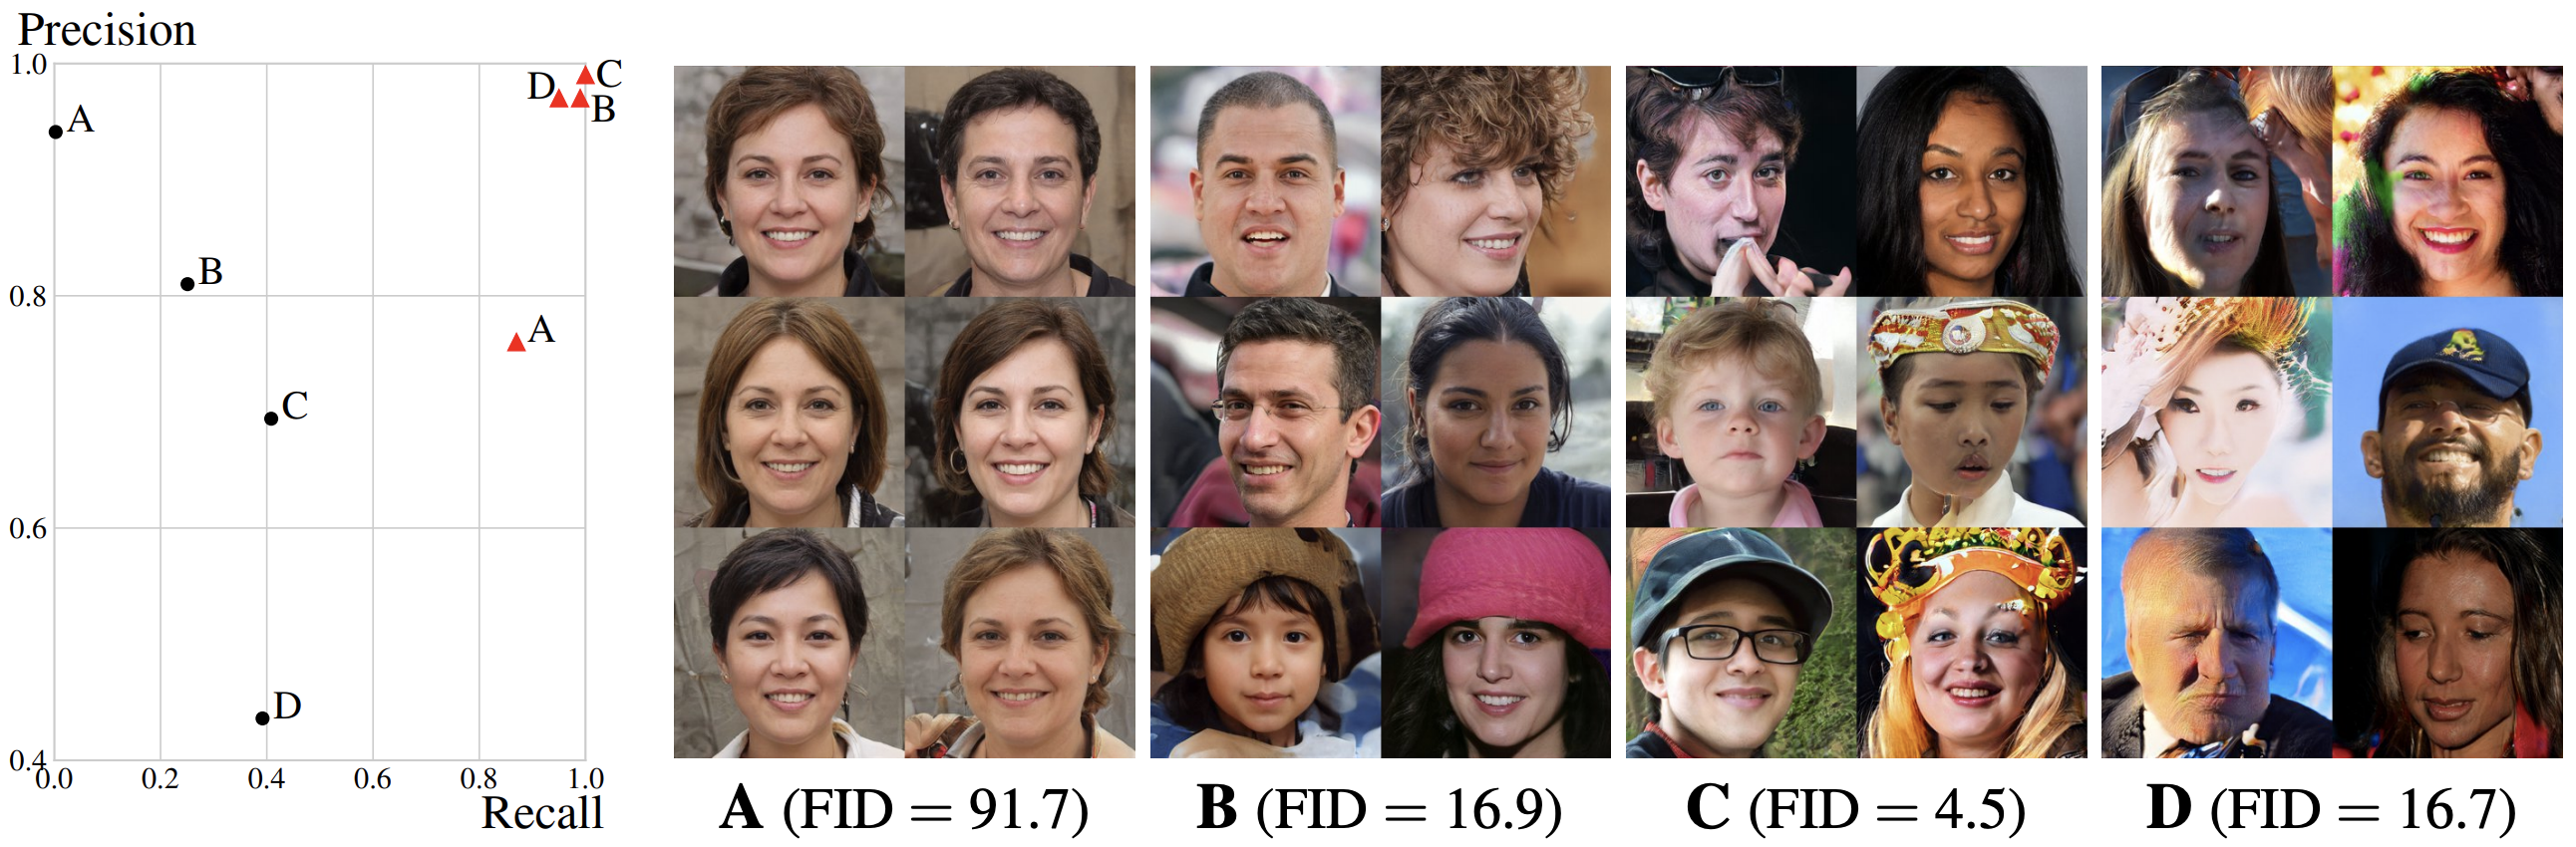
\includegraphics[width=\linewidth]{figs/pr_vs_fid}
	\end{figure}
	\begin{figure}
		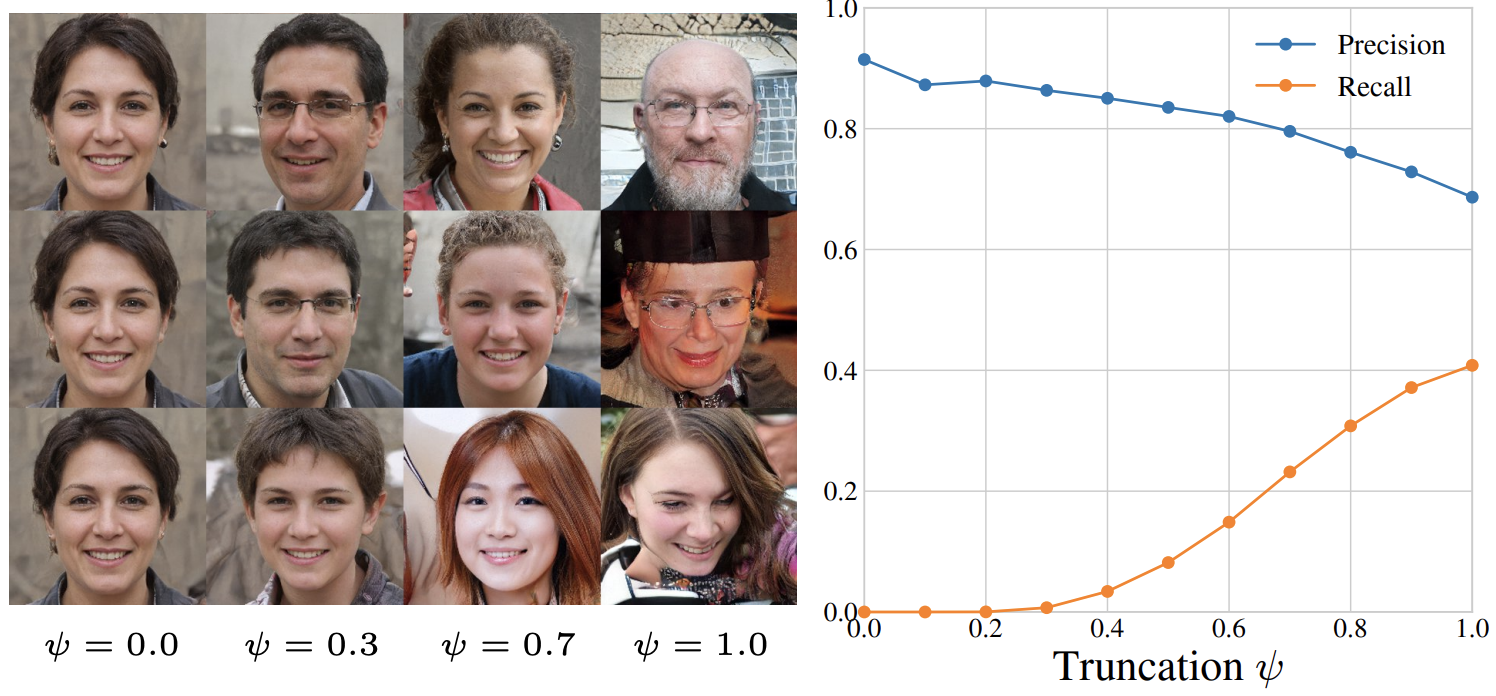
\includegraphics[width=0.75\linewidth]{figs/pr_truncation}
	\end{figure}
	\myfootnotewithlink{https://arxiv.org/abs/1904.06991}{Kynkäänniemi T. et al. Improved precision and recall metric for assessing generative models, 2019}
\end{frame}
%=======
\begin{frame}{Truncation trick}
	\begin{block}{BigGAN: truncated normal sampling}
		\vspace{-0.3cm}
		\[
			p(\bz | \psi) = \cN(\bz | 0, \bI) / \int_{-\infty}^\psi \cN(\bz' | 0, \bI) d\bz'
		\]
		Components of $\bz \sim \cN(0, \bI)$ which fall outside a predefined range are resampled.
	\end{block}
	
	\begin{block}{StyleGAN}
		\vspace{-0.2cm}
		\[
			\bz' = \hat{\bz} + \psi \cdot (\bz - \hat{\bz}), \quad \hat{\bz} = \bbE_{\bz} \bz
		\]
		\vspace{-0.2cm}
		\begin{itemize}
			\item Constant $\psi$ is a tradeoff between diversity and fidelity. 
			\item $\psi=0.7$ is used for most of the results.
		\end{itemize}
	\end{block}

	\myfootnote{\href{https://arxiv.org/abs/1809.11096}{Brock A., Donahue J., Simonyan K. Large Scale GAN Training for High Fidelity Natural Image Synthesis, 2018} \\
	\href{https://arxiv.org/abs/1812.04948}{Karras T., Laine S., Aila T. A Style-Based Generator Architecture for Generative Adversarial Networks, 2018}}
\end{frame}
%=======
\section{Langevin dynamic}
%=======
\begin{frame}{Langevin dynamic}
	\vspace{-0.4cm}
	\begin{block}{Statement}
		Let $\bx_0$ be a random vector. Then samples from the following dynamics
		\vspace{-0.3cm}
		\[
			\bx_{l + 1} = \bx_l + \frac{\eta}{2} \cdot \nabla_{\bx_l} \log p(\bx_l | \btheta) + \sqrt{\eta} \cdot \bepsilon, \quad \bepsilon \sim \cN(0, \bI).
		\]
		will come from $p(\bx | \btheta)$ (under mild regularity conditions, for small enough $\eta$ and large enough $l$).
	\end{block}
	\begin{minipage}{0.55\linewidth}
		\begin{itemize}
			\item Here we assume that we already have some generative model $p(\bx | \btheta)$.
			\item The density $p(\bx | \btheta)$ is a \textbf{stationary} distribution for the Markov chain. \\
			\item What do we get if $\bepsilon = \boldsymbol{0}$?
		\end{itemize}
	\end{minipage}%
	\begin{minipage}{0.4\linewidth}
		\begin{figure}
			\centering
			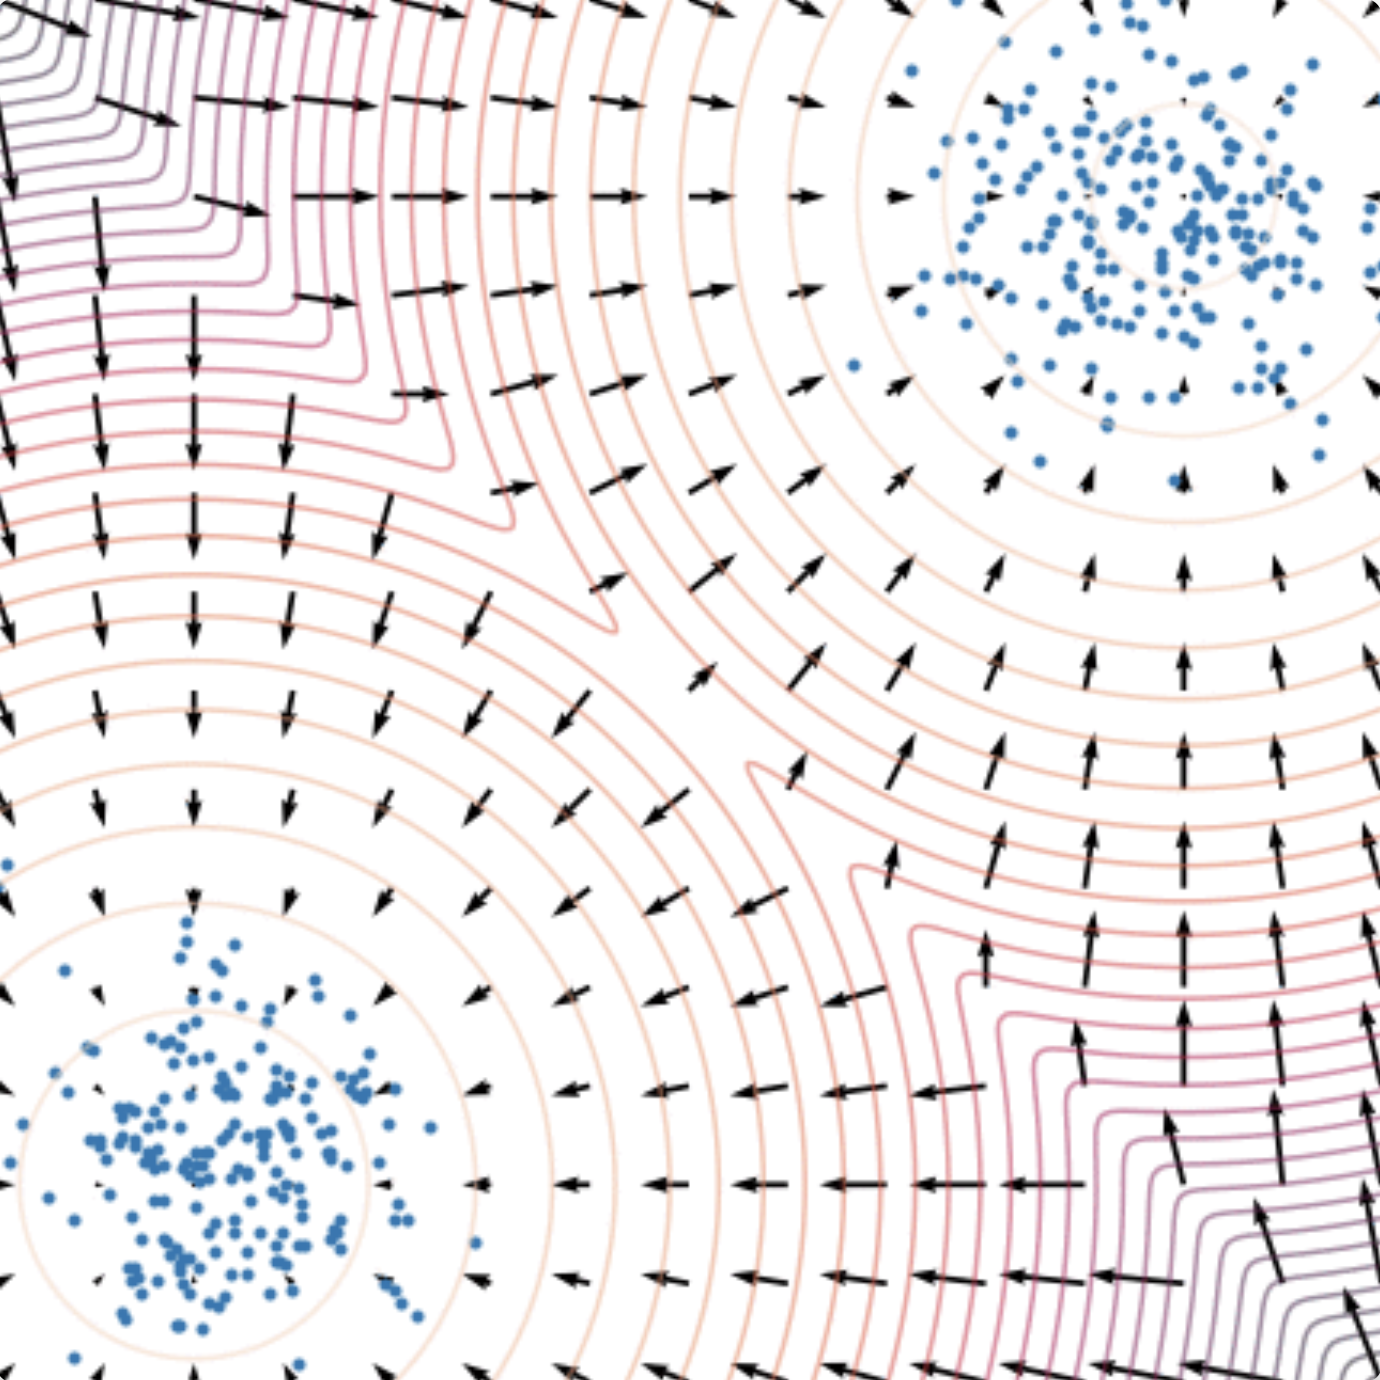
\includegraphics[width=0.9\linewidth]{figs/langevin_dynamic}
		\end{figure}
	\end{minipage}
	\myfootnotewithlink{https://yang-song.github.io/blog/2021/score/}{Song Y. Generative Modeling by Estimating Gradients of the Data Distribution, blog post, 2021} 
	\end{frame}
%=======
\begin{frame}{Energy-based models}
	\begin{block}{Langevin dynamic}
		\vspace{-0.3cm}
		\[
			\bx_{l + 1} = \bx_l + \frac{\eta}{2} \cdot \nabla_{\bx_l} \log p(\bx_l | \btheta) + \sqrt{\eta} \cdot \bepsilon, \quad \bepsilon \sim \cN(0, \bI).
		\]
		We are able to sample from the model using Langevin dynamics if we have $\nabla_{\bx}\log p(\bx| \btheta)$.
	\end{block}
	\begin{block}{Unnormalized density}
		\vspace{-0.2cm}
		\[
			p(\bx | \btheta) = \frac{\hat{p}(\bx | \btheta)}{Z_{\btheta}}, \quad \text{where } Z_{\btheta} = \int \hat{p}(\bx | \btheta) d \bx
		\]
		\vspace{-0.3cm}
		\begin{itemize}
			\item $\hat{p}(\bx | \btheta)$ is any non-negative function. \\
			\item If we use the reparametrization $\hat{p}(\bx | \btheta) = \exp(-f_{\btheta}(\bx))$, we remove the non-negativite constraint.
		\end{itemize}
		\[
			\nabla_{\bx} \log p(\bx | \btheta) = \nabla_{\bx} \log \hat{p}(\bx | \btheta) - \nabla_{\bx} \log Z_{\btheta} = \nabla_{\bx} \log \hat{p}(\bx | \btheta)
		\]
		The gradient of the normalized density equals to the gradient of the unnormalized density.
	\end{block}
\end{frame}
%=======
\section{Score matching}
%=======
\begin{frame}{Score matching}
	\begin{block}{Score function}
		\vspace{-0.3cm}
		 \[
			 \bs_{\btheta}(\bx) = \nabla_{\bx}\log p(\bx| \btheta)
		 \]
		\vspace{-0.5cm} 
	\end{block}
	\begin{block}{Langevin dynamic}
		If we find the score function $\bs_{\btheta}(\bx) = \nabla_{\bx}\log p(\bx| \btheta)$ we will be able to sample from the model using Langevin dynamic. 
		\[
			\bx_{l + 1} = \bx_l + \frac{\eta}{2} \cdot {\color{violet}\nabla_{\bx_l} \log p(\bx_l | \btheta)} + \sqrt{\eta} \cdot \bepsilon = \bx_l + \frac{\eta}{2} \cdot  {\color{violet}\bs_{\btheta}(\bx_l)} + \sqrt{\eta} \cdot \bepsilon.
		\] 
		\vspace{-0.5cm} 
	\end{block}
	\begin{block}{Fisher divergence}
		\vspace{-0.5cm}
		\begin{multline*}
			D_F(\pi, p) = \frac{1}{2}\bbE_{\pi}\bigl\| \nabla_{\bx}\log p(\bx| \btheta) - \nabla_\bx \log \pi(\bx) \bigr\|^2_2 = \\ 
			= \frac{1}{2}\bbE_{\pi}\bigl\| \bs_{\btheta}(\bx) - \nabla_\bx \log \pi(\bx) \bigr\|^2_2 \rightarrow \min_{\btheta}
		\end{multline*}
		\vspace{-0.3cm}
	\end{block}
	\myfootnotewithlink{https://yang-song.github.io/blog/2021/score/}{Song Y. Generative Modeling by Estimating Gradients of the Data Distribution, blog post, 2021}
\end{frame}
%=======
\begin{frame}{Score matching}
	\begin{block}{Fisher divergence}
		\vspace{-0.3cm}
		\[
			D_F(\pi, p) = \frac{1}{2}\bbE_{\pi}\bigl\| \bs_{\btheta}(\bx) - \nabla_\bx \log \pi(\bx) \bigr\|^2_2 \rightarrow \min_{\btheta}
		\]
		\vspace{-0.5cm}
	\end{block}
	\begin{figure}
		\centering
		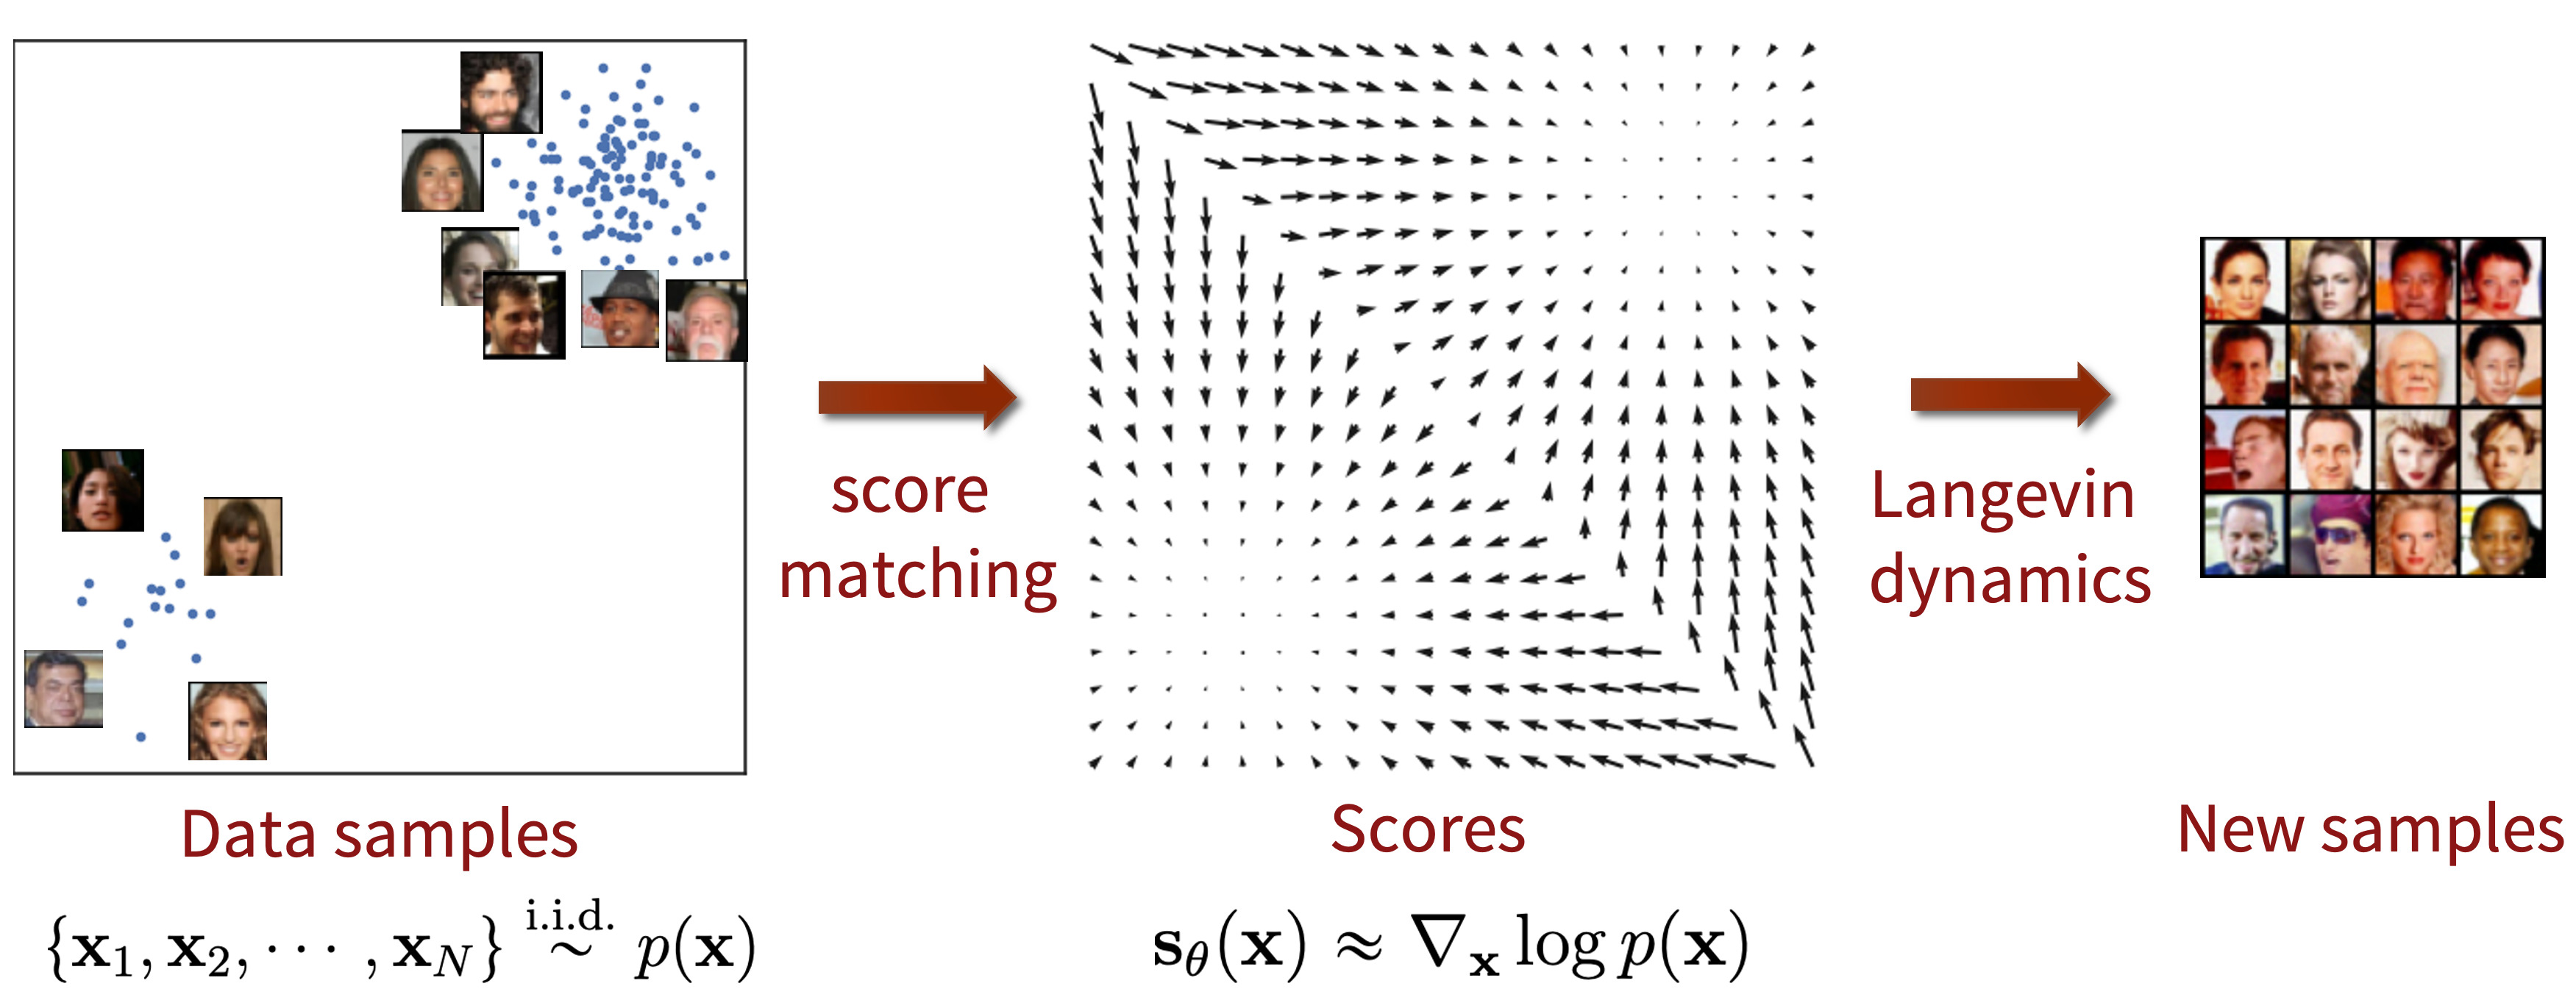
\includegraphics[width=\linewidth]{figs/smld}
	\end{figure} 
	\textbf{Problem:} We do not know $\nabla_\bx \log \pi(\bx)$.
	\myfootnotewithlink{https://yang-song.github.io/blog/2021/score/}{Song Y. Generative Modeling by Estimating Gradients of the Data Distribution, blog post, 2021}
\end{frame}
%=======
\begin{frame}{Summary}
	\begin{itemize}
		\item We need a measure of quality for the implicit models (like GANs). 
		\vfill 
		\item Frechet Inception Distance is the most popular metric for the implicit models evaluation. 
		\vfill
		\item Maximum Mean Discrepancy tries to fix some of the FID drawbacks.
		\vfill
		\item Precision-recall allow to select model that compromises the sample quality and the sample diversity.	
		\vfill 
		\item Truncation tricks help to select model with the compromised samples: diverse and sharp.
		\vfill
		\item Langevin dynamic allows to sample from the generative model using the gradient of the log-likelihood.	
		\vfill
		\item Score matching proposes to minimize the Fisher divergence to get the score function.
	\end{itemize}
\end{frame}
%=======
\end{document} 